\documentclass{article}
\usepackage{picinpar,graphicx}
\graphicspath{{/home/li/图片/}}
\usepackage{cite}
\usepackage{multicol}
\usepackage{lscape}
\author{Qingyun Li}
\date{May 5, 2018}
\title{CNN}
\begin{document}
\maketitle
 \par In Wiki, CNN is explained that in machine learning, a convolutional neural network (CNN, or ConvNet) is a class of deep, feed-forward artificial neural networks that has successfully been applied to analyzing visual imagery. We can see its structure at Fig.~\ref{CNN}, it includes the convolutional layer and pooling layer. CNNs use relatively little pre-processing compared to other image classification algorithms. This means that the network learns the filters that in traditional algorithms were hand-engineered. This independence from prior knowledge and human effort in feature design is a major advantage. Now, They have applications in image and video recognition, recommender systems\cite{van2013deep} and natural language processing\cite{collobert2008unified}.
\begin{figure}[htbp]
\begin{minipage}{1\linewidth}
\centering
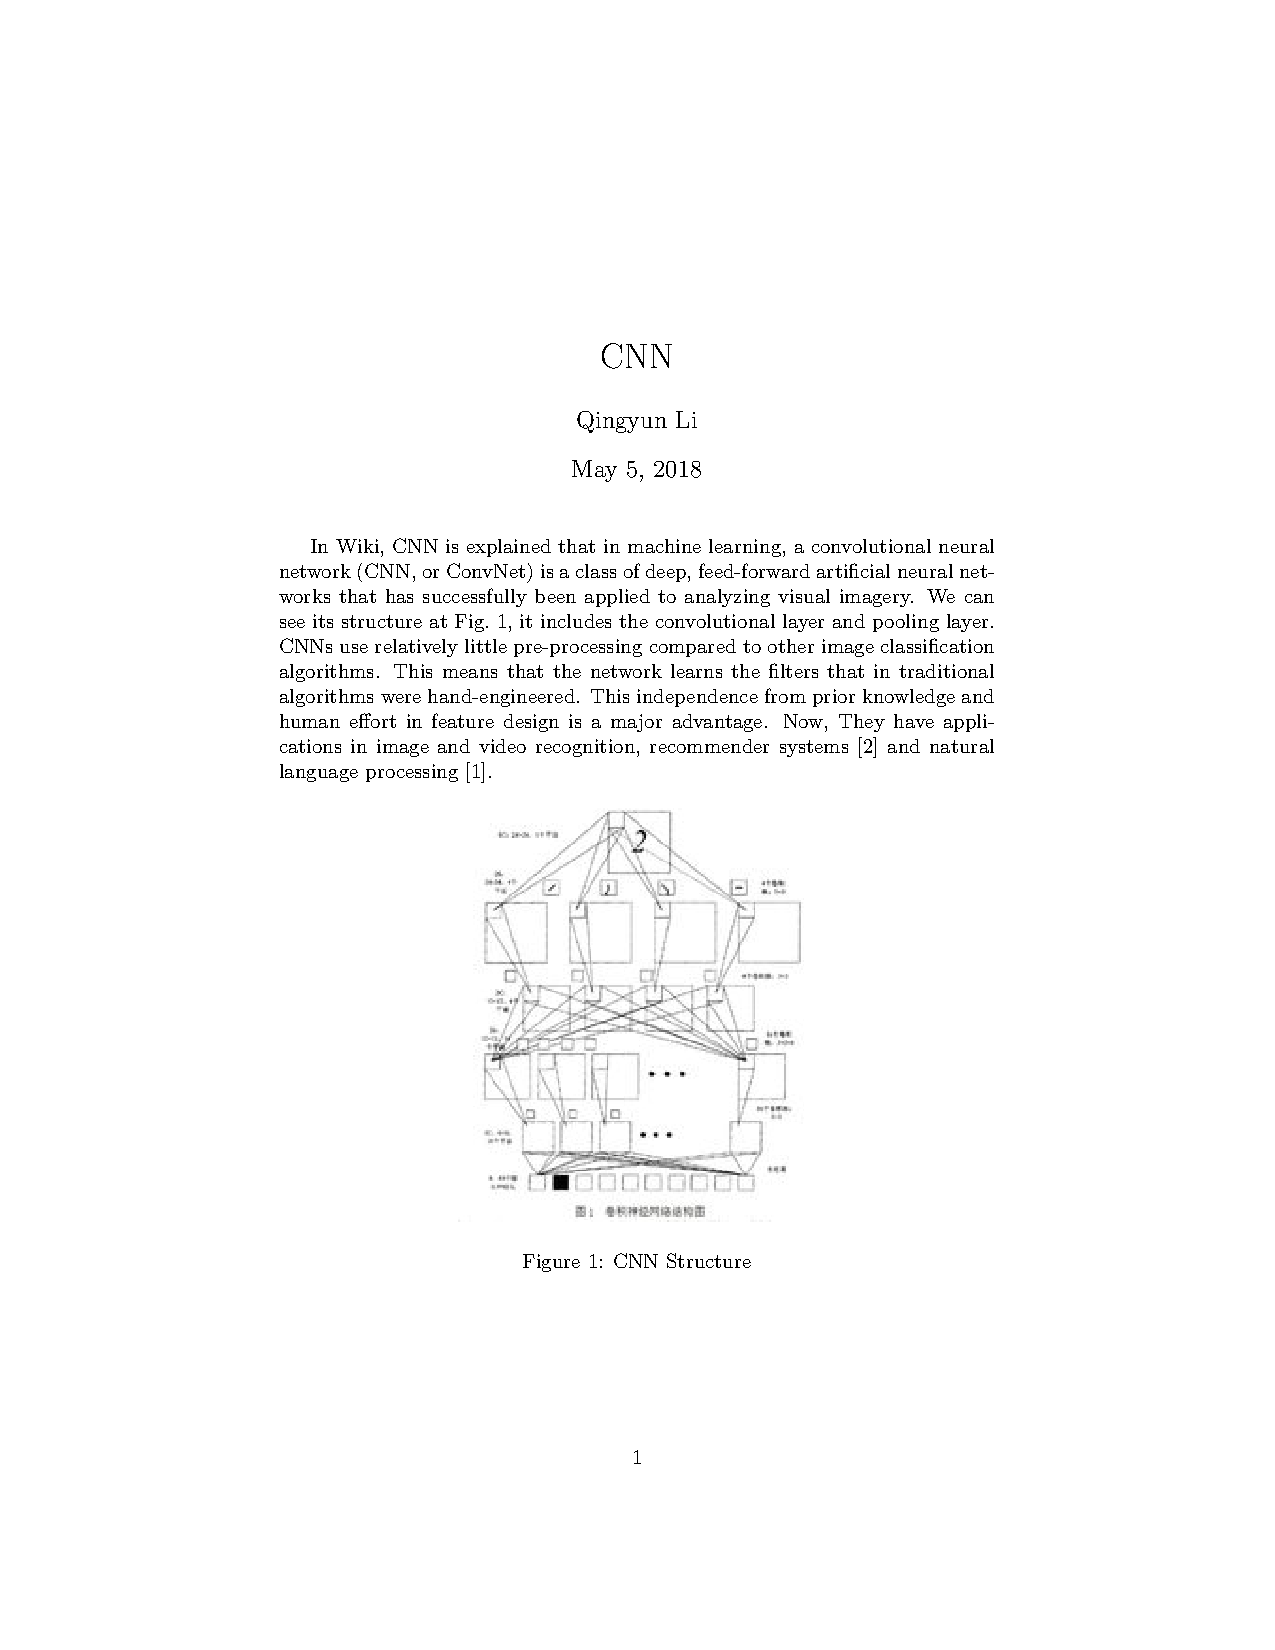
\includegraphics[width=0.5\linewidth]{CNN.png}\\
\caption{CNN Structure}\label{CNN} 
\end{minipage}
\end{figure}
\bibliographystyle{plain}
\bibliography{single}
\end{document}